\section{Model setup \& data}

The COSMO model in CLimate Mode (COSMO-CLM) has been designed both for operational numerical weather prediction and scientific applications on the meso-\(\beta\) and meso-\(\gamma\) scale. The limited-area atmospheric model receives boundary and initial conditions from a driving host model, or, in our case study, from ERA-Interim reanalysis data (resolution of 0.75°). Time integration relies on a third-order Runge-Kutta scheme. The number of both vertical and soil levels is equal to 10. The model equations are formulated in rotated geographical coordinates to reduce the effect of varying grid cell size. Parametrization for grid-scale clouds and precipitation is based on a Kessler-type bulk formulation, which uses specific grouping of particles into broad categories of water substance (e.g., cloud water) that interact by various microphysical processes. The implemented cloud ice scheme allows explicit representation of ice clouds. While vertical turbulent diffusion parametrization is based on a prognostic equation for turbulent kinetic energy, as far as I am concerned, no subgrid-scale (deep) convection scheme is included by default\footnote{\code{itype\_conv} undefined in model namelists}.   
The time step has been set to \SI{150}{\s} for all resolutions. For further information about the COSMO model please refer to \textcite{schaettler2021}.


\begin{table}
	\centering
	\begin{tabular}{cccc}
		\toprule
		Experiment name & Resolution [°] & Grid & Spacing [\(\approx\)km] \\
		\midrule
		02° & 0.2 & 280 \(\times\) 230 & 25 \\
		05° & 0.5 & 100 \(\times\) 80  & 65 \\
		1° & 1 & 56 \(\times\) 46      & 130 \\
		\bottomrule
	\end{tabular}
	\caption{COSMO-CLM simulations of this study}
	\label{tab:sims}
\end{table}

The study is composed of three COSMO-CLM simulations during January 1990, as introduced in \cref{tab:sims}. This period of time has been chosen as grid definition files and appropriately scaled boundary conditions were already available. \Cref{fig:regionbox} displays the mean precipitation within the entire model domain, however, structures of \enquote{unphysical} values are clearly visible at the edges, where interpolation between model output and constraining boundary conditions alters the results. In the following, the region of interest is reduced to the area of the red rectangle. It is notable that the 05°-simulation region seems to be cropped in the north and east compared to the other simulations. This is due to an erroneous value in the number of grid points during grid definition, but will not affect the results as the region of analysis is still sufficiently large. 

\begin{figure}
	\centering
	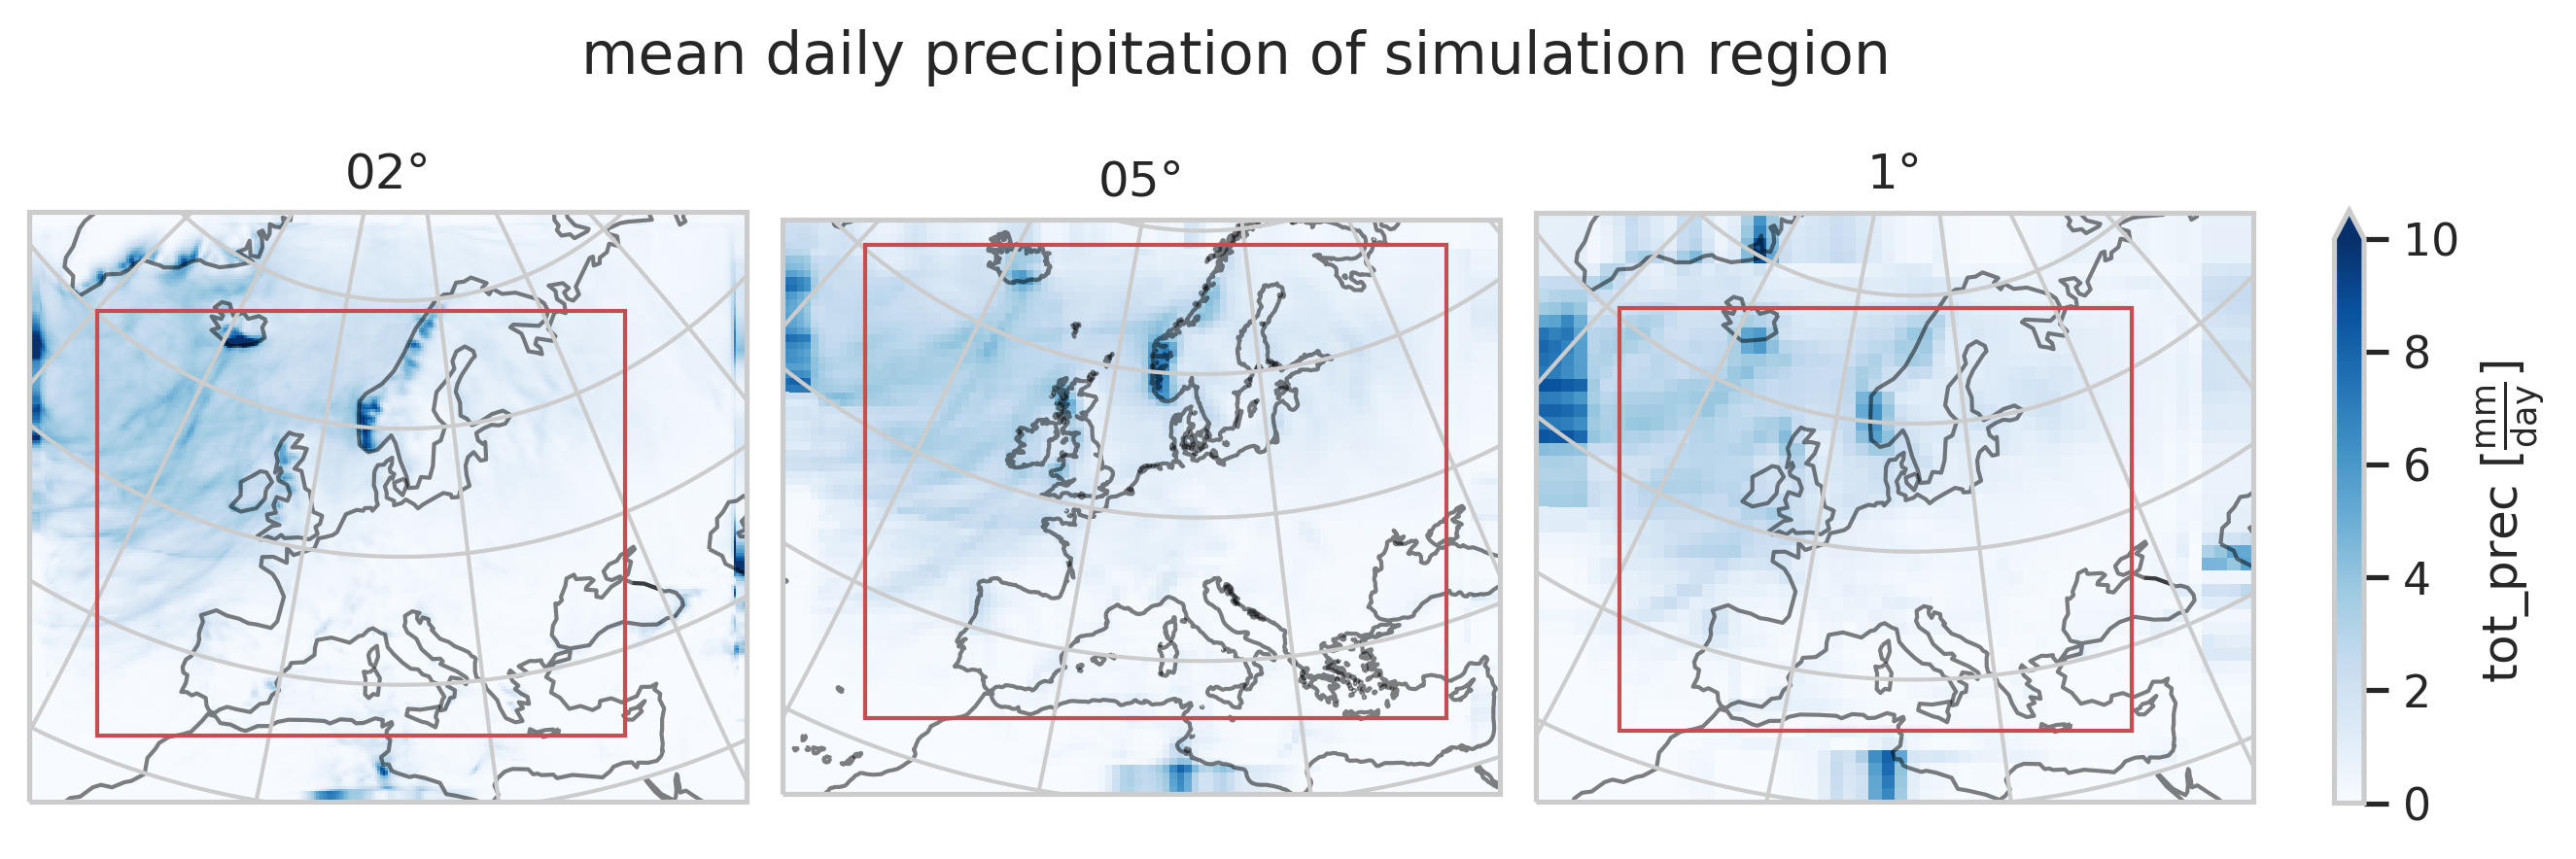
\includegraphics[width=\figwidth]{../figs/1-regionbox.png}
	\caption{Spatial domains of simulations. Red rectangle indicates area of analysis. Please note that here and in the following figures pointed ends of a colourbar indicate out-of-range values.}
	\label{fig:regionbox}
\end{figure}
	
In this study, ERA5 reanalysis data produced by the ECMWF serves as a reference. Although also a model product themselves, reanalyses assimilate observational records and thus are a reasonable choice to compare simulation output with. ERA5 data is provided on a 0.28° grid, however, here, the data is remapped to a 0.2° rotated grid to be able to cut the same region as in the COSMO-CLM simulations (see \cref{fig:regionbox}).

The shell script for data processing, python code for re-creating all figures as well as further comments can be found in the related online repository\footnote{\url{https://gitlab.met.fu-berlin.de/rw0064fu/mwu-gridres}}. Much data processing has been realized by using \textit{Climate Data Operators} of \textcite{schulzweida2022}. 